\chapter{Конструкторский раздел}	
В конструкторской части разработано программное обеспечение, а также формально описаны применяемые алгоритмы.

\section{Схемы алгоритмов визуализации трехмерной сцены}
\subsection{Алгоритм, использующий z-буфер}
На рисунках~\ref{fig:z_buf_2} представлена схема алгоритма с использованием z-буфера. В алгоритме выполняется разложение треугольника в растр, после чего вычисляется глубина полученного пикселя. Вычисленная глубина сравнивается с записанной в z-буфере, в зависимости от результата может быть выполнено обновление z-буфера.  

\begin{figure}[H]
	\centering
	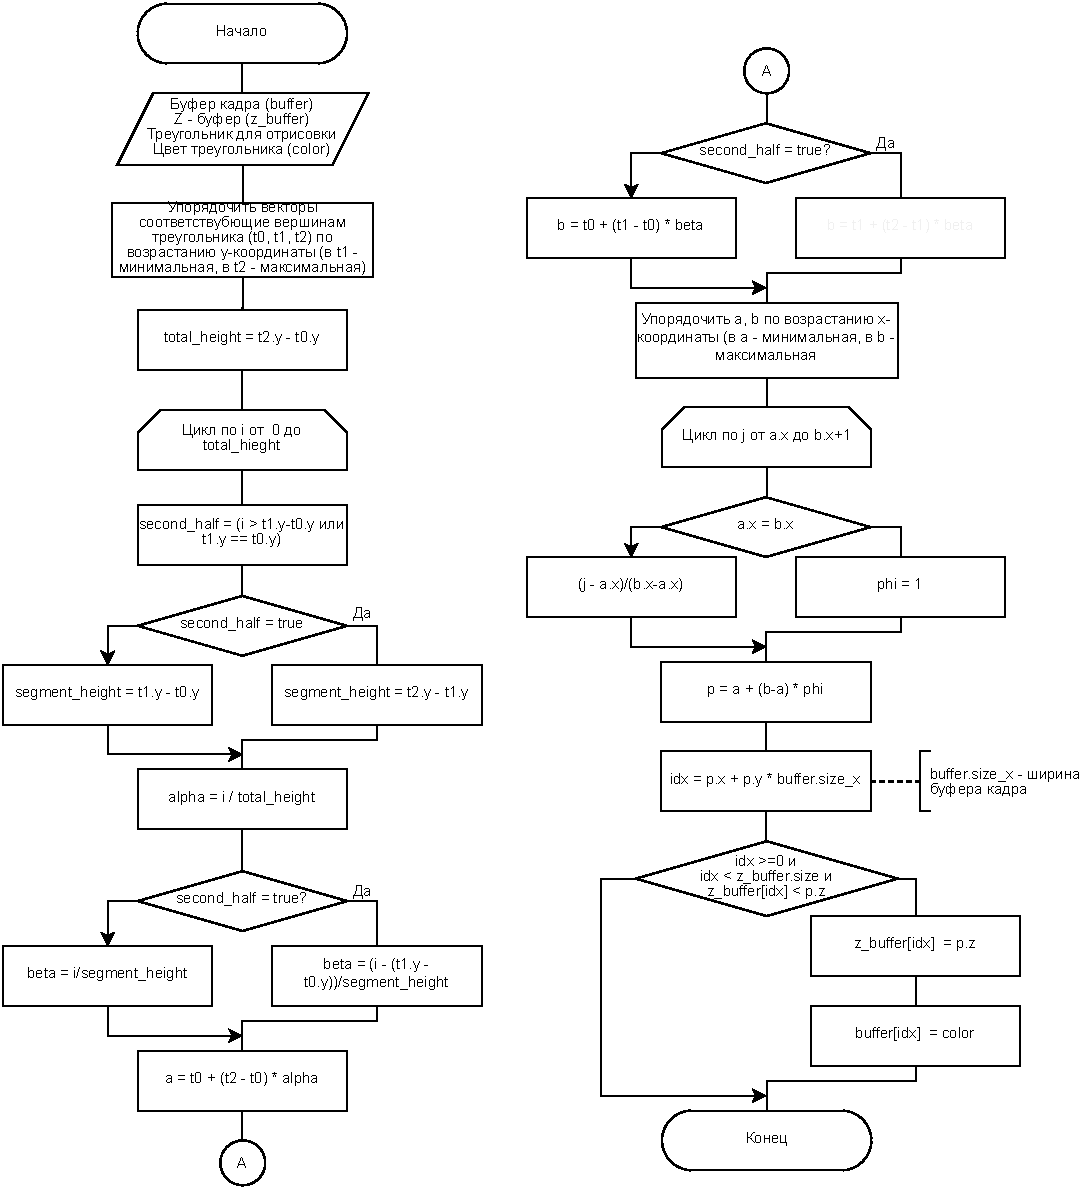
\includegraphics[width=1.0\textwidth, page=1]{assets/img/z-bufer-full.pdf}   
	\caption{Схема алгоритма с использованием z-буфера.}
	\label{fig:z_buf_2}
\end{figure}

\subsection{Алгоритм поведения газов}

На рисунке~\ref{fig:Navie-Stocks} представлена схема алгоритма поведения газа на основе уравнений Навье---Стокса. 
\begin{figure}[H]
	\centering
	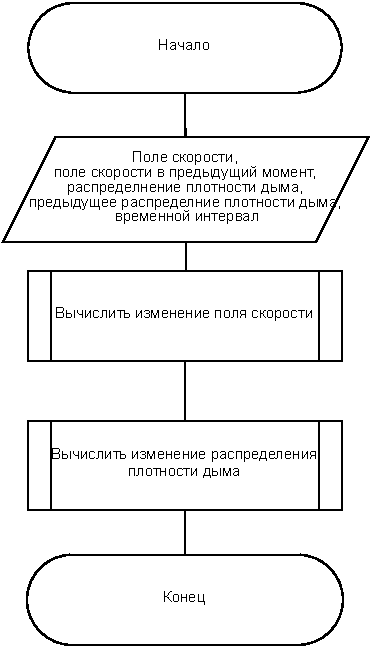
\includegraphics[width=0.7\textwidth, page=1]{assets/img/Naive_stocks.pdf}   
	\caption{Схема алгоритма на основе уравнения Навье---Стокса.}
	\label{fig:Navie-Stocks}
\end{figure}

На рисунке~\ref{fig:dens_step} представлена схема алгоритма обновления распределения плотности дыма.

\begin{figure}[H]
	\centering
	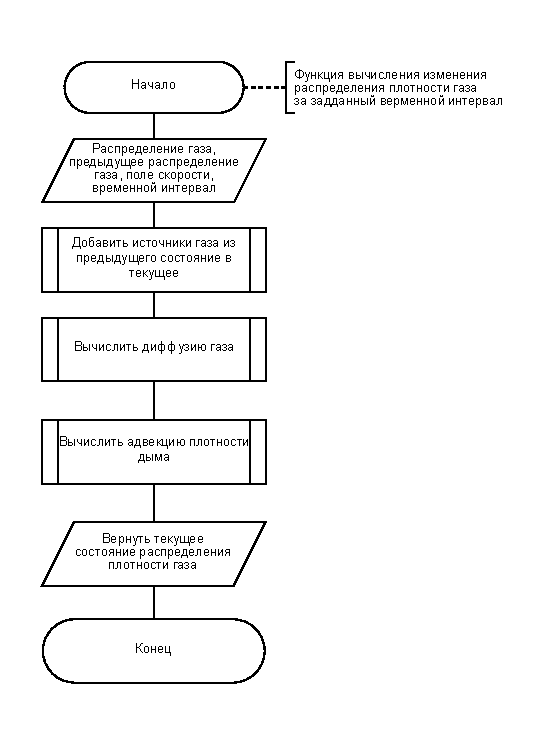
\includegraphics[width=0.6\textwidth, page=1]{assets/img/dens_step.pdf}   
	\caption{Схема алгоритма обновления распределения плотности дыма.}
	\label{fig:dens_step}
\end{figure}

На рисунке~\ref{fig:vel_step} представлена схема алгоритма обновления поля скорости.

\begin{figure}[H]
	\centering
	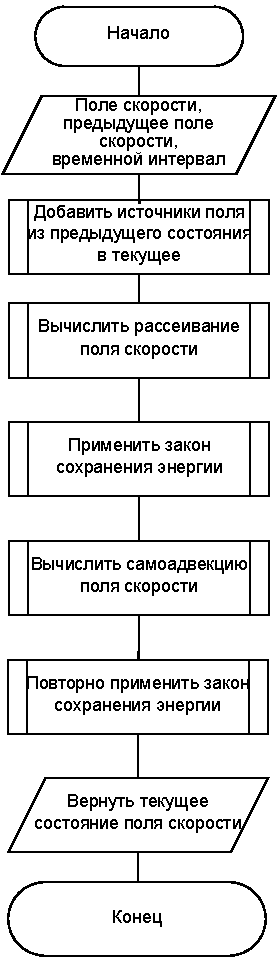
\includegraphics[width=0.4\textwidth, page=1]{assets/img/velocity_step.pdf}   
	\caption{Схема алгоритма обновления поля скорости.}
	\label{fig:vel_step}
\end{figure}

На рисунке~\ref{fig:add_src} представлена схема алгоритма добавления источников в систему, используемая как в алгоритме обновления поля скорости, так и в алгоритме обновления распределения плотности дыма.

\begin{figure}[H]
	\centering
	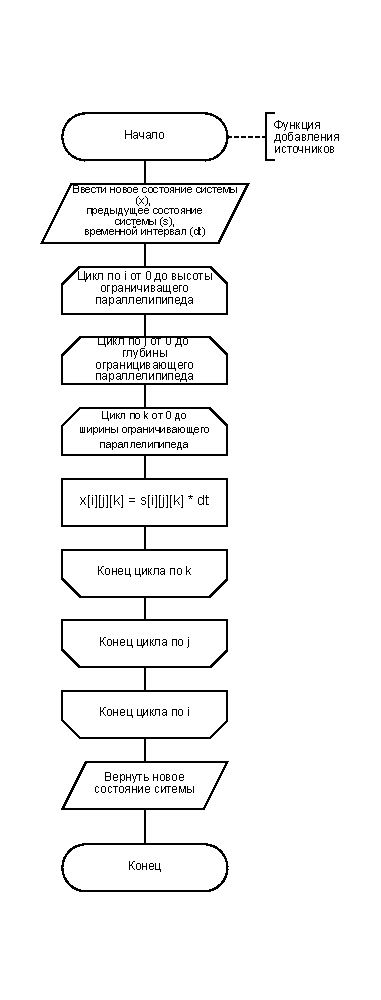
\includegraphics[width=1.0\textwidth, page=1]{assets/img/add_source.pdf}
	\caption{Схема алгоритма добавления источников в систему.}
	\label{fig:add_src}
\end{figure}

На рисунке~\ref{fig:diffuse} представлена схема алгоритма вычисления диффузии (рассеивания), используемого для обновления поля скорости и распределения плотности газа. В обоих случаях под диффузией предполагается обмен ячейки ограничивающего параллелепипеда плотностью или скоростью с соседними по граням ячейками. Пример для двумерной симуляции представлен на рисунке~\ref{fig:diffusion}. Для трехмерного случая вычисление нового распределения плотности сводится к решению системы уравнений вида~\ref{eq:diffusion}, относительно неизвестных $x$. При этом рассматривается изменение распределения плотности в обратном временном порядке, т.~е. для ячейки $i, j, k$ находится плотность, которая при распространении назад во времени дает плотности предыдущего распределения. Для решения СЛАУ применяется итеративный метод Гаусса-Зейделя, алгоритм которого представлен на рисунке~\ref{fig:lin_solve}.

\begin{equation}
	\label{eq:diffusion}
	x_{0_{i,j,k}} = x_{i,j,k} - D \cdot (x_{i-1,j, k}+x_{i+1,j, k}+x_{i,j-1, k}+x_{i,j+1, k}+x_{i, j, k-1}+x_{i, j, k-1}-6*x_{i,j, k})
\end{equation}
где:
\begin{itemize}
	\item $x_0$ --- исходное распределение плотности;
	\item $x$ --- вычисляемое распределение плотности;
	\item $D$ --- коэффициент диффузии.
\end{itemize}

\begin{figure}[H]
	\centering
	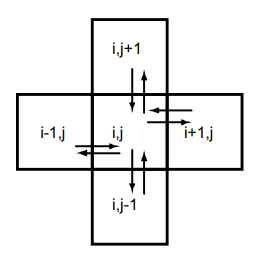
\includegraphics[width=0.4\textwidth, page=1]{assets/img/diffusion.png}   
	\caption{Пример диффузии для двумерной симуляции.}
	\label{fig:diffusion}
\end{figure}

\begin{figure}[H]
	\centering
	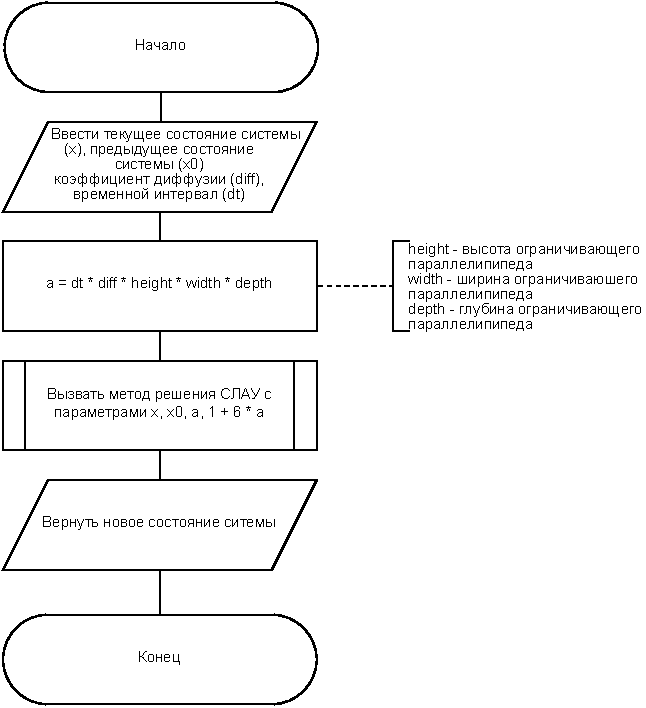
\includegraphics[width=1.0\textwidth,page=1]{assets/img/diffuse.pdf}
	\caption{Схема алгоритма вычисления диффузии (рассеивания).}
	\label{fig:diffuse}
\end{figure}

\begin{figure}[H]
	\centering
	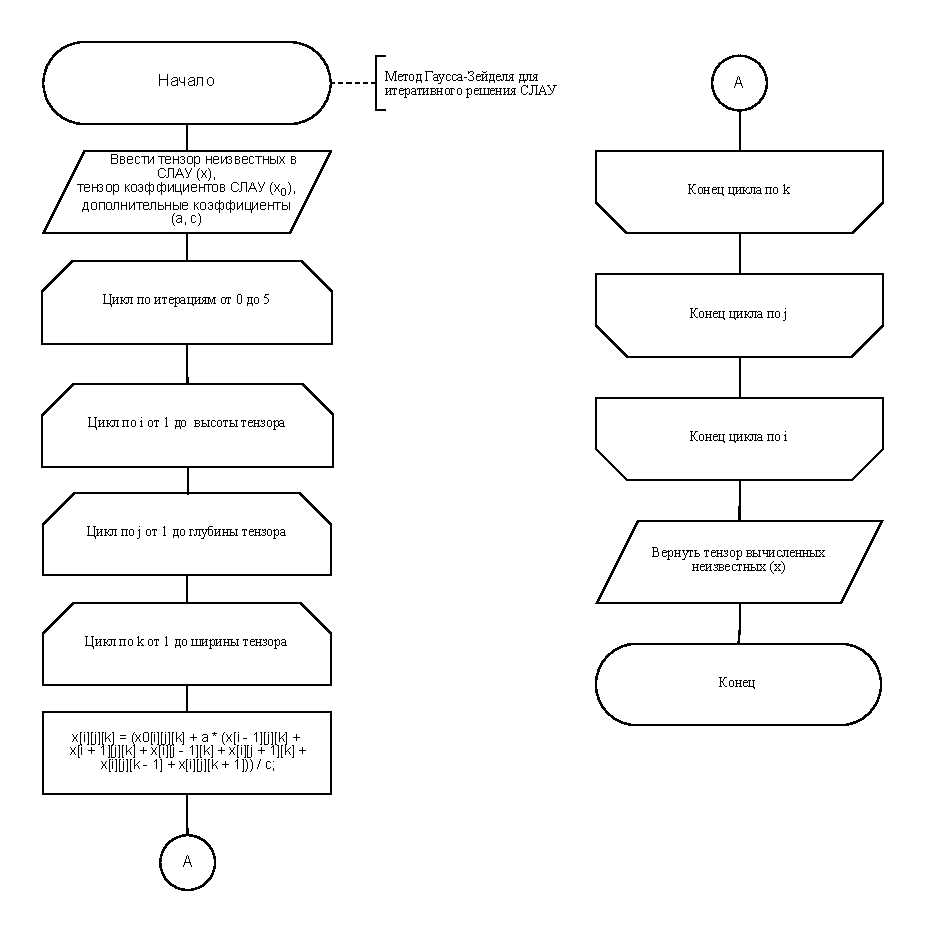
\includegraphics[width=1.0\textwidth,page=1]{assets/img/gauss-zeidel.pdf}
	\caption{Схема алгоритма решения СЛАУ.}
	\label{fig:lin_solve}
\end{figure}

На рисунке~\ref{fig:advect} представлена схема алгоритма вычисления адвекции и самоадвекции для распределение плотности и поля скорости соответственно. Для вычисления адвекции также используется подход обратного временного распространения. Для значений, которые в итоге находятся в центре ячейки ограничивающего параллелепипеда, линейной интерполяцией определяются доли значений соседних ячеек перенесенных полем скорости за единичный временной шаг. На рисунке~\ref{fig:advect_idea} проиллюстрирована идея вычисления адвекции для двумерной симуляции. Таким образом исходная точка, откуда была перенесена плотность за один временной интервал вычисляются по формуле~\ref{eq:advect_1}. 

\begin{equation}
	\label{eq:advect_1}
	\vec{p_0} = \vec{p} - \vec{v} \cdot \Delta t
\end{equation}
где:
\begin{itemize}
	\item $\vec{p_0}$~---~вычисленная исходная точка;
	\item $\vec{p}$~---~точка соответствующая центру ячейки, для которой вычисляется новое значение плотности;
	\item $\vec{v}$~---~скорость в точке, соответствующей центру ячейки, для которой вычисляется новое значение плотности;
	\item $\Delta t$~---~временной интервал.
\end{itemize}

Для каждой координаты полученной исходной точки определяется отрезок интерполяции с помощью формул~\ref{eq:advect_2} (пример приведен для x-координаты). 
\begin{equation}
	\label{eq:advect_2}
	\begin{matrix}
		x_0 = \floor{x} \\
		x_1 = x_0 + 1
	\end{matrix}
\end{equation}
где:
\begin{itemize}
	\item $x$~---~x-координата вычисленной исходной точки;
	\item $x_0$, $x_1$~---~границы отрезка интерполяции.
\end{itemize}

Далее для каждой координаты определяются расстояния до границ отрезка интерполяции по формулам~\ref{eq:advect_3} (пример также приведен для x-координаты).
\begin{equation}
	\label{eq:advect_3}
	\begin{matrix}
		k_{x0} = p_{0_x} - x_0 \\
		k_{x1} = 1 - k_{x0}
	\end{matrix}
\end{equation}
где:
\begin{itemize}
	\item $p_{x_0}$~---~
\end{itemize}
\begin{figure}[H]
	\centering
	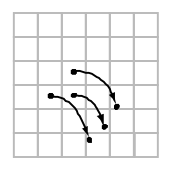
\includegraphics[width=0.4\textwidth,page=1]{assets/img/advect.png}
	\caption{Пример вычисления адвекции. Стрелками показано обратное распространение плотности во времени.}
	\label{fig:advect_idea}
\end{figure}

\begin{figure}[H]
	\centering
	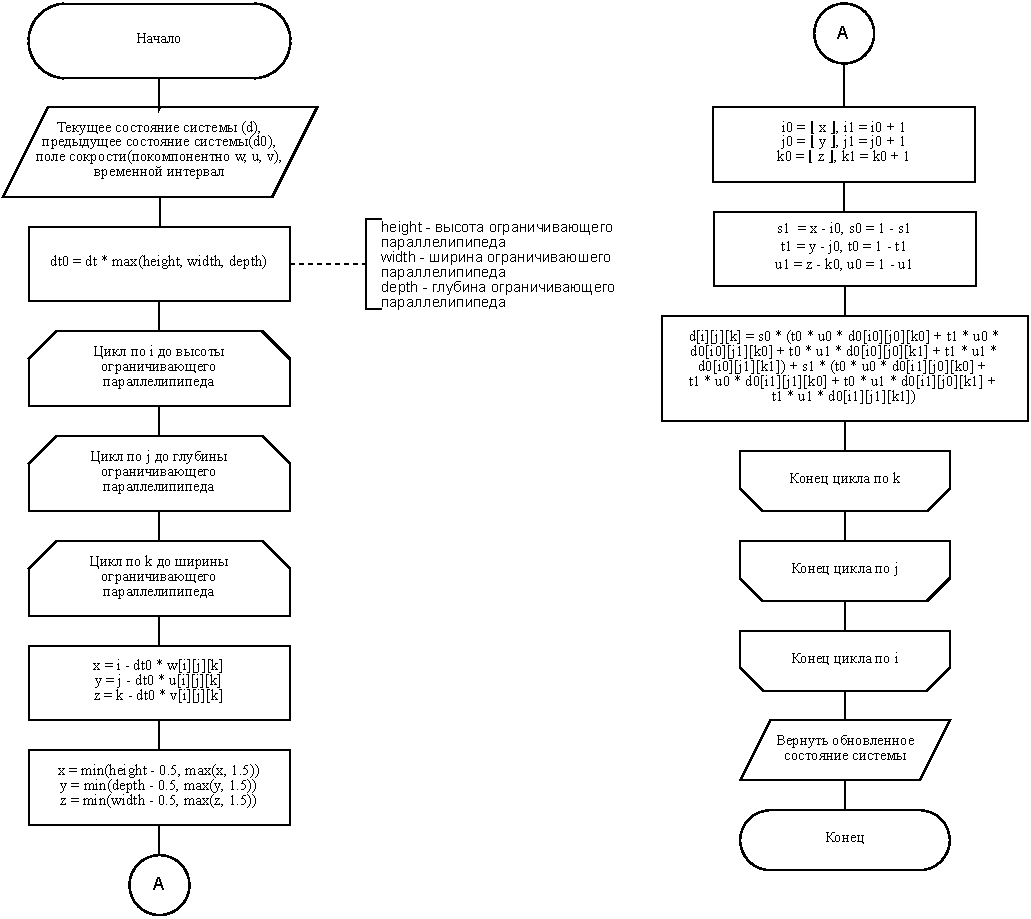
\includegraphics[width=1.0\textwidth,page=1]{assets/img/advect.pdf}
	\caption{Схема алгоритма вычисления адвекции.}
	\label{fig:advect}
\end{figure}

На рисунке~\ref{fig:project} представлена схема алгоритма применения закона сохранения массы к полю скорости. Так как несжимаемость является неотъемлемой частью реальных газов, необходимо, чтобы данный закон выполнялся для итогового поля скорости. В соответствии с декомпозицией Ходжа, каждое поле скорости является суперпозицией несжимаемого поля и градиентной составляющей, как показано на рисунке~\ref{fig:hodge}. Для получения поля, которое будет сохранять массу необходимо в каждой точке вычесть из существующего поля градиент. Таким образом, задача сводится к нахождения градиента в точке, для чего можно решить систему линейных уравнений методом, использованным ранее. Закон сохранения массы применяется дважды лишь потому, что вычисление адвекции происходит точнее, когда для поля скорости выполняется данный закон~\cite{stam}.

\begin{figure}[H]
	\centering
	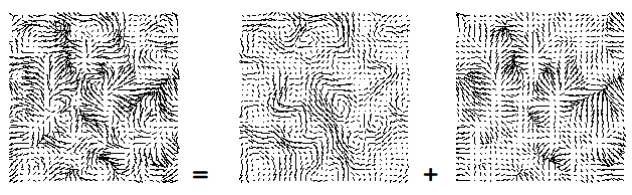
\includegraphics[width=0.7\textwidth,page=1]{assets/img/hodge.png}
	\caption{Декомпозиция Ходжа. После знака равенства: слева --- несжимаемая составляющая, справа --- градиентная.}
	\label{fig:hodge}
\end{figure}

\begin{figure}[H]
	\centering
	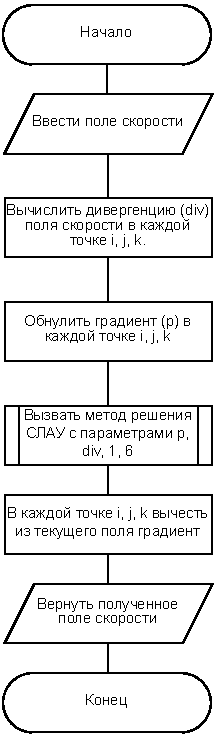
\includegraphics[width=1.0\textwidth,page=1]{assets/img/project.pdf}
	\caption{Схема алгоритма применения закона сохранения массы.}
	\label{fig:project}
\end{figure}

\section{Диаграмма классов}

На рисунке~\ref{fig:uml} представлена UML-диаграмма классов программного обеспечения.

\begin{figure}[H]
	\centering
	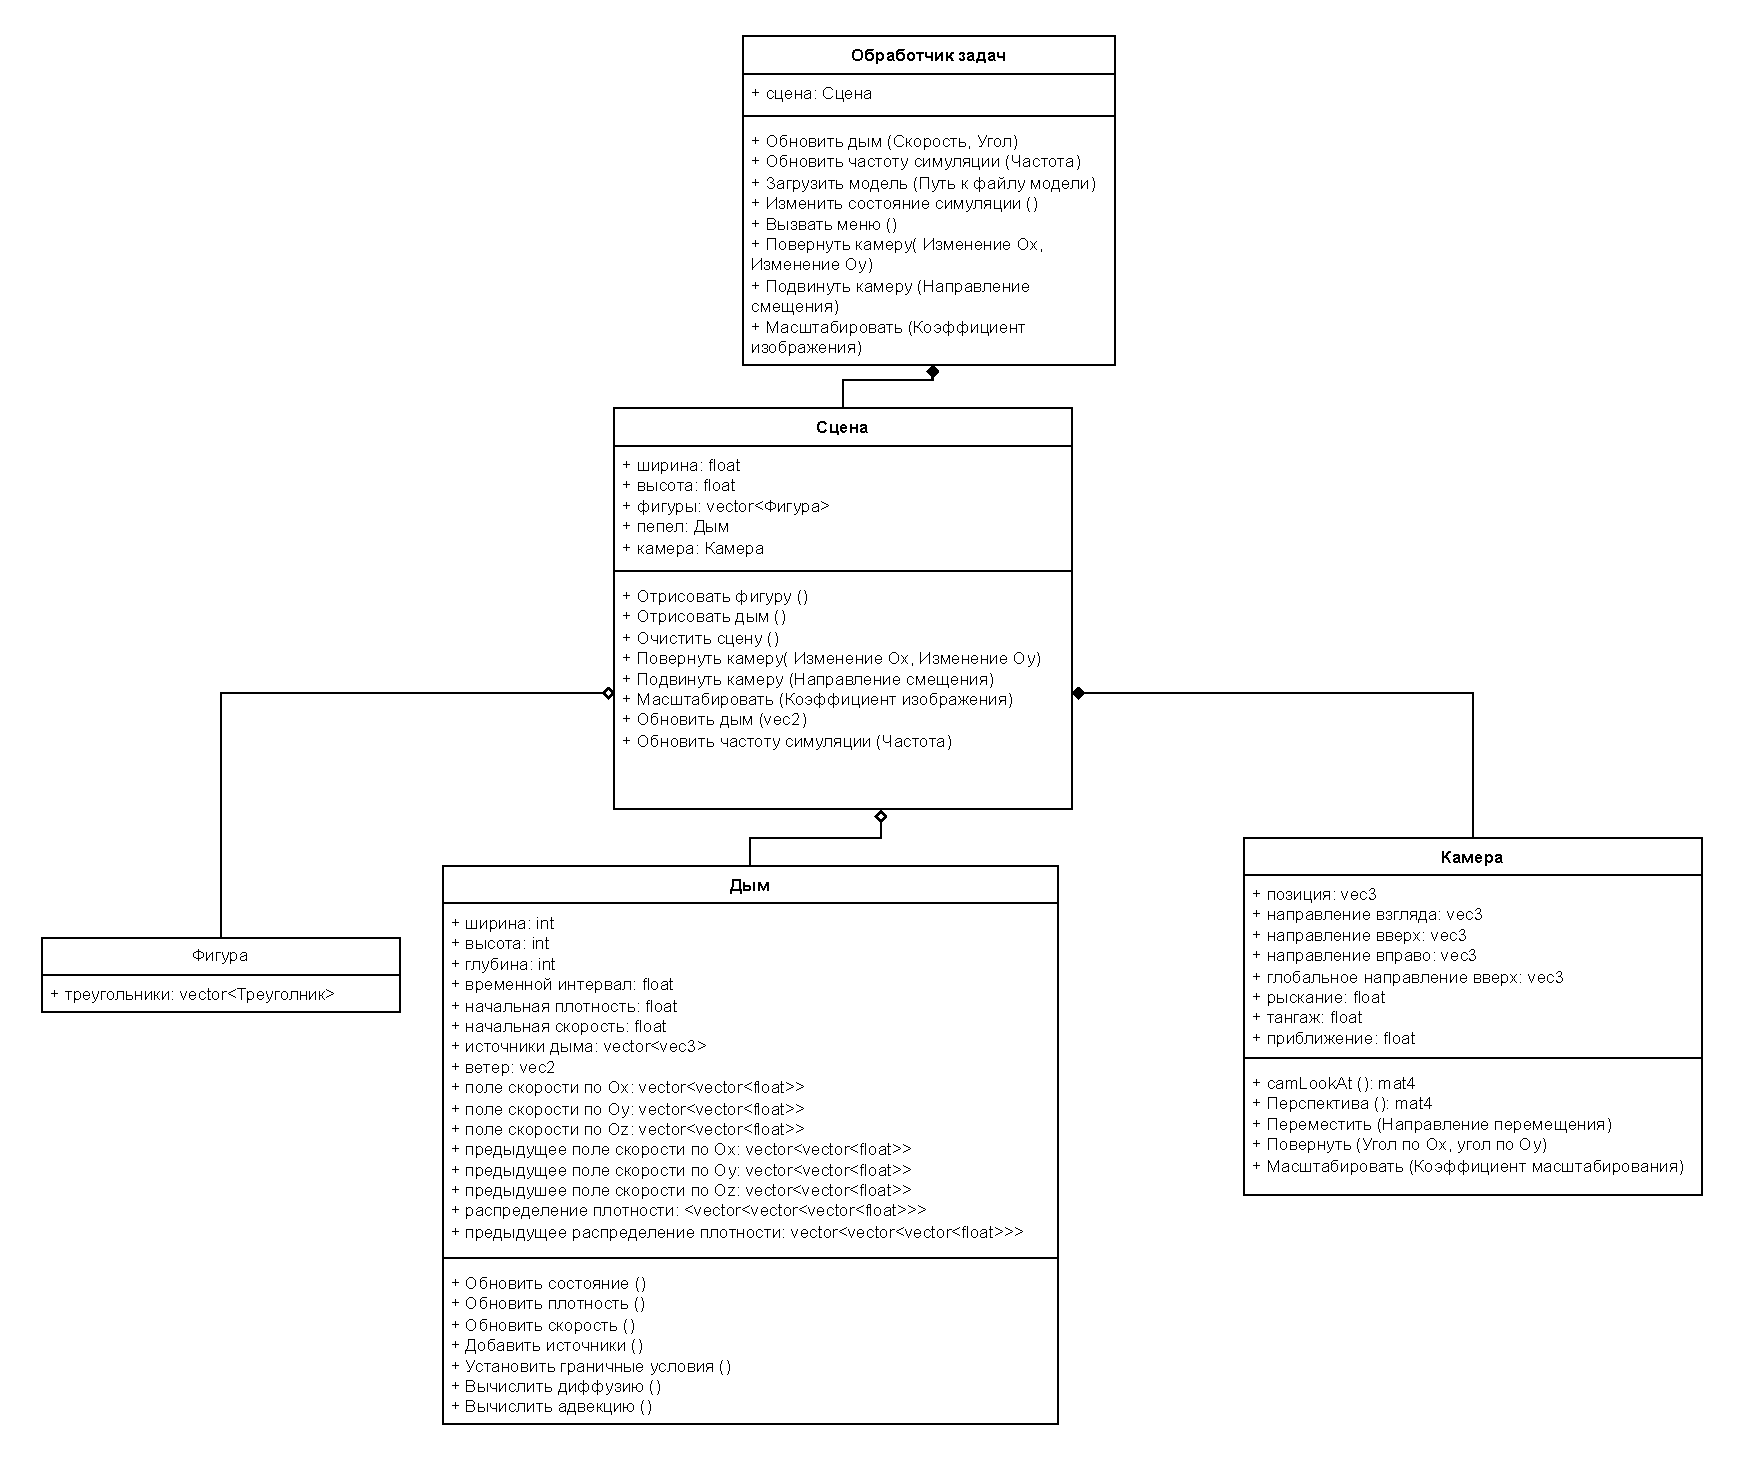
\includegraphics[width=0.9\textwidth,page=1]{assets/img/smoke_uml.pdf}
	\caption{UML-диаграмма классов.}
	\label{fig:uml}
\end{figure}

\section*{Вывод}
В разделе спроектировано разрабатываемое программное обеспечение для визуализации извержения вулкана, приведены схемы алгоритмов и UML-диаграмма классов ПО.
